\documentclass[]{article}
\usepackage[utf8]{inputenc}
\usepackage[english]{babel}
\usepackage{graphicx}
\usepackage{hyperref}
\usepackage{appendix}
\hypersetup{
	colorlinks=true,
	linkcolor=blue,
	filecolor=magenta,      
	urlcolor=cyan,
}
\usepackage{mathtools}
\usepackage{float}   %this package is for placing graphs and tables in where the TeX is
\graphicspath{{images/}{../images/}}

\usepackage{blindtext}

\usepackage{subfiles}
\usepackage{verbatim}
\providecommand{\EqDir}{Equations}
\providecommand{\RefDir}{References}

\usepackage{apacite}


\title{Replication of Aiyagari(1994)}
\author{Zixuan Huang and Mingzuo Sun}
\date{}

\begin{document}
\linespread{2}
\maketitle




The paper we replicated is "Uninsured Idiosyncratic Risk and Aggregate Saving" by S. Rao  \cite{1994}. The paper was published in The Quaterly Journal of Economics, Vol. 109, No. 3 (Aug., 1994). Besides this document, you can also find the corresponding notebook \href{run:../Aiyagari1994QJE.ipynb}{here}, which contains concrete steps of our replication.

\section{Abstract}
The paper modifies standard growth model to include precautionary saving motives and liquidity constraints.The paper also examines the impact of the introduction of a particular kind of uninsurable idiosyncratic risk on the aggregate saving rate; the importance of asset trading to individuals; and the relative inequality of the wealth and income distributions. 

\section{Introduction}
The paper wants to provide an exposition of models whose aggregate behavior is the result of market interaction among a large number of agents subject to idiosyncratic shocks. Moreover, another goal of this paper is to use such a model to study the quantitative importance of individual risk for aggregate saving.\\

The paper mainly has five features: Endogenous heterogeneity, aggregation, infinite horizons, exogenous borrowing constraint, and general equilibrium. i.e. interest rate is endogenously determined since in a steady state equilibrium the capital per capita must equal the per capita asset holdings of consumers, and the interest rate must equal the net marginal product of capital. 

\section{Related Literature}
The model in Aiyagari(1994) originates from Bewley model and a subsequent literature Zeldes (1989), Deaton (1991), Carroll (1992), and puts these kinds of models into a general equilibrium context. These models all share the same key components as mentioned in the previous part. And they are used to study the following topics:
\begin{itemize}
	\item How much of observed wealth inequality does a particular choice of uninsurable idiosyncratic income uncertainty explain? 
	\item In this model, what is the fraction of aggregate savings due to the precautionary motive? 
	\item In this model, what are the re-distributional implications of various policies?
\end{itemize}

\section{Model}
\subsection{Individual's Problem}

\begin{align}
	\max E_0\left(\sum_{t=0}^\infty \beta^t U(c_t)\right)\\
	\text{s.t.}\\
	c_t+a_{t+1}=wl_{t}+(1+r)a_t \\
	c_t\geq0\\
	a_t\geq-\phi
\end{align} \\
where $\phi$ (if positive) is the limit on borrowing; $l_t$ is assumed to be i.i.d with bounded support given by $[l_{min},l_{max}]$, with $l_{min}>0$; $w$ and $r$ represent wage and interest rate respectively.

Let $\hat{a}_t \equiv a_t+\phi$ and $z_t \equiv wl_t+(1+r)\hat{a}_t-r\phi$, where $z_t$ can be interpreted as total resources of the agent at date $t$ respectively. 
Then the Bellman equation is as follows:
\begin{align}
$k_{jt+1}=(1-\delta)k_{jt}+i_{jt}$
\end{align}

Consequently, Euler equation is: 
\begin{align}
	1= R\beta E_{t-1}[\{c_t[R[m_{t-1}-c_{t-1}]/Gn_t + v_t]Gn_t/c_{t-1}\}^{-\rho}]
\end{align}

Solve the model, the decision rule can be written as: 
\begin{align}
	\hat{a}_{t+1}=A(z_t,\phi,w,r)
\end{align}

And the law of transition would be:
\begin{align}
	z_{t+1}=wl_{t+1}+(1+r)A(z_t,\phi,w,r)-r\phi
\end{align}

\subsection{Firm's Problem}
\begin{align}
	\max F(K,L)-wL-rK
\end{align}
where $K$ is the aggregate capital, $L$ is the aggregate labor, $F(K,L)$ is the production function.

\subsection{General Equilibrium}
In the steady state, variables are time invariant and all markets are clear, i.e.,
\begin{itemize}
	\item $F_K(K,L) = r+\delta$ 
	\item $F_L(K,L) = w$
	\item $\int l_i di = L$
	\item $\int a_i di = K$	
\end{itemize}


\section{Model Specification, Parameters and Computation}
\subsection{Model specification and parameters}
We follow the parameters in Aiyagari(1994) for calibration. Parameters are listed in the table below. 
\subfile{Tables/Table_Parameters}

Production function is Cobb Douglas production function with the capital share taken to be $\alpha$
\begin{align}
	F(K,L) = K^\alpha L^{1-\alpha}
\end{align}

Utility function is CRRA utility function with the relative risk aversion coefficient $\mu$.\\

Finally, labor endowment shocks follow an AR process.
\begin{align}
\log(l_t)=\rho\log(l_{t-1})+\sigma(1-\rho^2)^{\frac{1}{2}}\epsilon_{t}, \ \epsilon_t \sim N(0,1)   
\end{align}



\subsection{Computation}
This notebook uses \href{http://www.econforge.org/dolark/}{EconForge/Dolark} toolkit to describe the results and reproduce the tables in the linked paper. And you can our application of this toolkit for this paper in the \href{run:../Aiyagari1994QJE.ipynb}{notebook} we created.


\section{Key Results}
\subsection{Aggregate Saving Rates}
Table \ref{table:1} shows the comparison between aggregate saving rates calculated by us and those in Aiyagari(1994). The results in Aiyagari(1994) are shown in section \ref{Appendix} of this document.\\

Our results are highly similar to but a bit different fom those in Aiyagari(1994). This is very likely because we use a different discrete-valued Markov Chain(MC) to approximate the AR process of individuals' idiosyncratic income shock. In our replication, three grid points (i.e. three MC states), which is set by default in $\texttt{Dolo}$ and $\texttt{Dolark}$, are used to simulate the AR process, whereas this number is seven in Aiyagari(1994).
\begin{table}[H]
	\scalebox{.7}{\begin{tabular}{rrrrrr}
\hline
    &   Risk Averse Coefficient &   Variance of Labor Shocks &   Serial Correlation &   Saving Rate &   Saving Rate\_Aiyagari \\
\hline
  0 &                         1 &                        0.2 &                  0   &         24.28 &                  23.67 \\
  1 &                         1 &                        0.2 &                  0.3 &         24.28 &                  23.73 \\
  2 &                         1 &                        0.2 &                  0.6 &         24.33 &                  23.82 \\
  3 &                         1 &                        0.2 &                  0.9 &         24.38 &                  24.14 \\
  4 &                         1 &                        0.4 &                  0   &         24.4  &                  23.87 \\
  5 &                         1 &                        0.4 &                  0.3 &         24.48 &                  24.09 \\
  6 &                         1 &                        0.4 &                  0.6 &         24.65 &                  24.5  \\
  7 &                         1 &                        0.4 &                  0.9 &         24.75 &                  25.47 \\
  8 &                         3 &                        0.2 &                  0   &         25.66 &                  23.71 \\
  9 &                         3 &                        0.2 &                  0.3 &         25.73 &                  23.91 \\
 10 &                         3 &                        0.2 &                  0.6 &         26.08 &                  24.25 \\
 11 &                         3 &                        0.2 &                  0.9 &         28.38 &                  25.51 \\
 12 &                         3 &                        0.4 &                  0   &         26.8  &                  24.44 \\
 13 &                         3 &                        0.4 &                  0.3 &         27.17 &                  25.22 \\
 14 &                         3 &                        0.4 &                  0.6 &         28.35 &                  26.71 \\
 15 &                         3 &                        0.4 &                  0.9 &         36.53 &                  31    \\
 16 &                         5 &                        0.2 &                  0   &         26.69 &                  23.83 \\
 17 &                         5 &                        0.2 &                  0.3 &         26.83 &                  24.19 \\
 18 &                         5 &                        0.2 &                  0.6 &         27.41 &                  24.86 \\
 19 &                         5 &                        0.2 &                  0.9 &         31.64 &                  27.36 \\
 20 &                         5 &                        0.4 &                  0   &         28.35 &                  25.22 \\
 21 &                         5 &                        0.4 &                  0.3 &         28.94 &                  26.66 \\
 22 &                         5 &                        0.4 &                  0.6 &         30.8  &                  29.37 \\
 23 &                         5 &                        0.4 &                  0.9 &         44.49 &                  37.63 \\
\hline
\end{tabular}}
	\caption{Aggregate Saving Rate}
	\label{table:2}
\end{table}


\subsection{Wealth Distribution}
The following figure shows the wealth distribution, where the x-axis represents the level of wealth and the y-axis represents the share of population.
\begin{figure}[H]
	\centering
	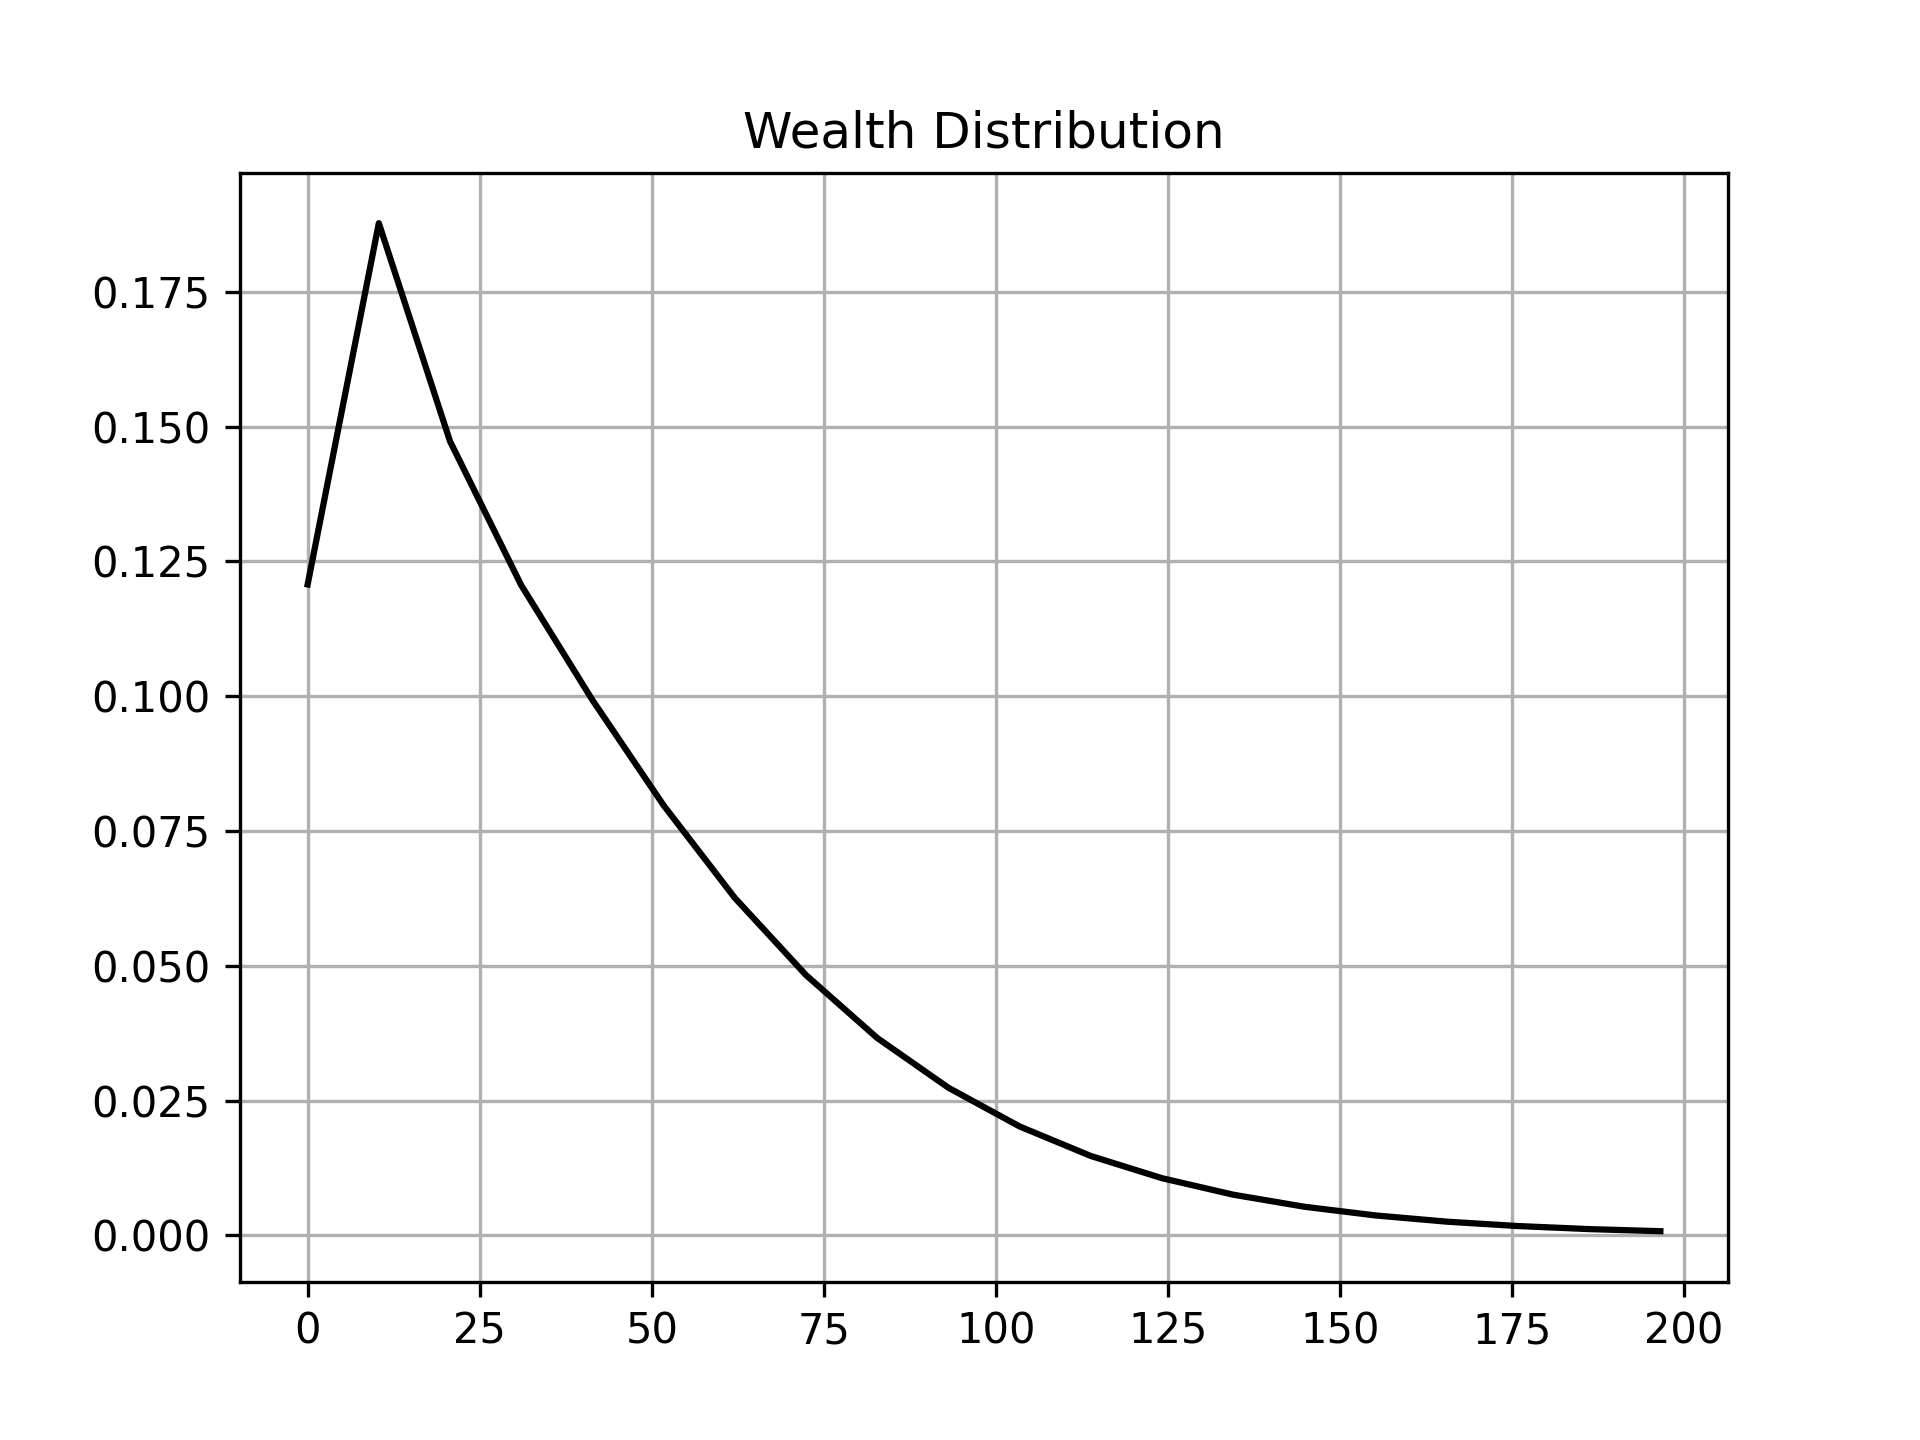
\includegraphics{Figures/Figure_WealthDistribution}
	\label{figure:1}
\end{figure}
\newpage 

\section{Appendix}{\label{Appendix}}
	\subfile{Appendix/Appendix}
\newpage 

\bibliographystyle{apacite}
\bibliography{References/Aiyagari1994}

\end{document}
